\documentclass[11pt]{article}
\usepackage[scaled=0.92]{helvet}
\usepackage{geometry}
\geometry{letterpaper,tmargin=1in,bmargin=1in,lmargin=1in,rmargin=1in}
\usepackage[parfill]{parskip} % Activate to begin paragraphs with an empty line rather than an indent %\usepackage{graphicx}
\usepackage{amsmath,amssymb, mathrsfs, dsfont, stackrel}
\usepackage{tabularx}
\usepackage[font=footnotesize,labelfont=bf]{caption}
\usepackage{graphicx}
\usepackage{xcolor}
%\usepackage[linkbordercolor ={1 1 1} ]{hyperref}
%\usepackage[sf]{titlesec}
\usepackage{natbib}
\usepackage{../../Tianpei_Report}
%\usepackage{appendix}
%\usepackage{algorithm}
%\usepackage{algorithmic}

%\renewcommand{\algorithmicrequire}{\textbf{Input:}}
%\renewcommand{\algorithmicensure}{\textbf{Output:}}



\begin{document}
\title{Lecture 2: Causal Graphical Models}
\author{ Tianpei Xie}
\date{Sep. 8th., 2022 }
\maketitle
\tableofcontents
\newpage
\allowdisplaybreaks
\section{Directed Graphical Models}
Given a graph $\cG = (\cV, \cE)$, where $\cV$ is the set of vertices and $\cE \subset \cV \times \cV$ is the set of edges, a \emph{probabilistic graphical model (PGM)} defines a \emph{joint probability distribution} $p(x_1, \ldots, x_{m})$ that \underline{\emph{\textbf{factorizes}}} according to $\cG$. Here each variable $x_i$ corresponds to a node $v_i \in \cV$ and the existence of an edge $(s,t) \in \cE$ (or the \emph{\textbf{absence}} of an edge $(s,t)$) defines a \textbf{statistical dependency} (or \underline{\textbf{conditional independency}}) relation between $x_s$ and $x_t$.  

If the edge $(s, t) \in \cE$ is \textbf{directed} (referred $s\rightarrow t$), i.e. there is a distinction between $(s, t)$ and $(t, s)$, the corresponding graphical models are referred as \emph{{directed graphical models}}.  Note that since a sequence of directed edges defines a logic flow, a circle in the graph would create undesireable contradiction. Therefore, we assume that $\cG$ is a \textbf{directed acyclic graph (DAG)}, meaning
that every edge is directed, and that the graph contains no directed cycles. 

For any such DAG, we can define a \textbf{partial order} on the vertex set $\cV$ by the notion of \emph{ancestry}:  we say that node $s$ is an \emph{ancestor} of $u$ if there is a \emph{directed path} $(s,t_1,t_2,\ldots,t_k,u)$. This is referred as \textbf{\emph{topological ordering}}. Given a DAG, for each vertex $u$ and its parent set $\pi(u) = \set{s \in \cV: (s\rightarrow u) \in \cE }$, the conditional probability $p_s(x_s | x_{\pi(s)})$ is a \textbf{non-negative function} over $ (x_s, x_{\pi(s)})$ and is \textbf{normalized} for all $x_s$, i.e. $\int p_s(x_s | x_{\pi(s)}) dx_s = 1.$

The \textbf{directed graphical model} thus factorizes the joint distribution into a set of \emph{local functions} $\{p_s(x_s | x_{\pi(s)}): s\in \cV\}$ according to the ancestor relations defined in $\cG$
\begin{align}
p(x_1, \ldots, x_{m}) &= \prod_{s \in \cV}p_s(x_s | x_{\pi(s)}). \label{eqn: dag_graph_factorization}
\end{align} This class of models are also referred as \emph{\textbf{Bayesian networks}} \citep{koller2009probabilistic}.

\subsection{Conditional independence and d-separation}
\begin{figure}
\begin{minipage}[t]{0.5\linewidth}
  \centering
  \centerline{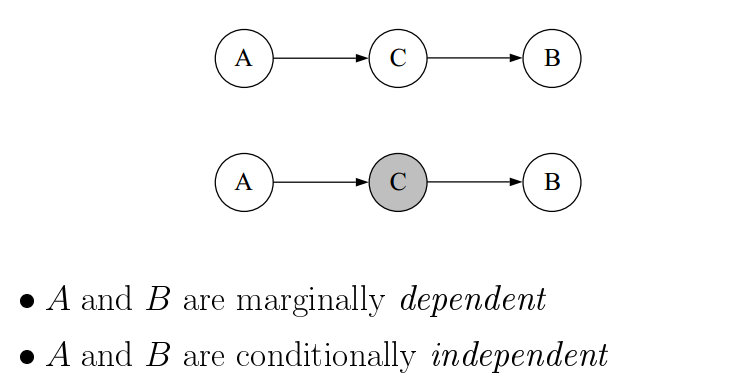
\includegraphics[scale = 0.32]{cond_indep_1.png}}
  \vspace{-5pt}
  \centerline{(a)}
\end{minipage}
\begin{minipage}[t]{0.5\linewidth}
  \centering
  \centerline{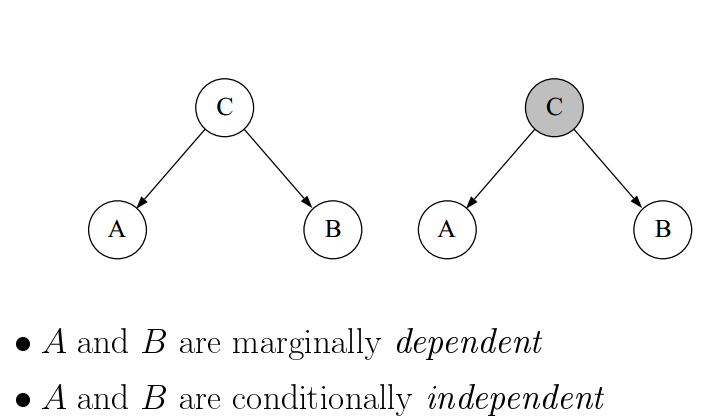
\includegraphics[scale = 0.3]{cond_indep_2.png}}
  \vspace{-5pt}
  \centerline{(b)}
\end{minipage}\\
\begin{minipage}[t]{0.5\linewidth}
  \centering
  \centerline{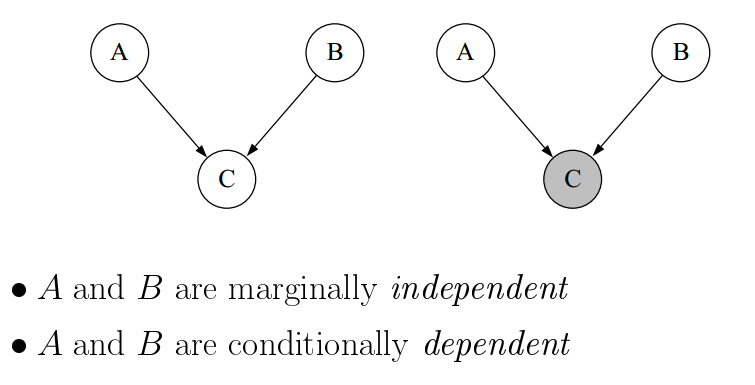
\includegraphics[scale = 0.35]{cond_indep_3.png}}
  \vspace{-5pt}
  \centerline{(c)}
\end{minipage}
\caption{\footnotesize{\textbf{The conditional independency structure in directed graph. The shaded nodes are observed. In (c), the variable $A$ and $B$ are marginally \emph{dependent} but conditionally \emph{independent} due to collider $C$. }}}
\label{fig: cond_indep}
\end{figure}

\begin{itemize}
\item 
\begin{definition} (\emph{\textbf{Pearl's d-separation}}) \citep{koller2009probabilistic, pearl2000causal, peters2017elements}\\
In a DAG $\cG$, a \emph{\textbf{path}} between nodes $i_1$ and $i_m$ is \underline{\textbf{\emph{blocked}}} by a set $S$ (with neither $i_1$ nor $i_m$ in $S$) whenever \emph{there is} a node $i_k$, such that \textbf{one} of the following two possibilities holds:
\begin{enumerate}
\item $i_k \in S$ and 
\begin{align*}
i_{k−1} \rightarrow i_k \rightarrow  i_{k+1} \\
\text{or }\quad i_{k−1} \leftarrow i_k \leftarrow  i_{k+1} \\
\text{or }\quad i_{k−1} \leftarrow i_k \rightarrow i_{k+1}
\end{align*}

\item neither $i_k$ nor any of its descendants is in $S$ and
\begin{align*}
i_{k−1} \rightarrow i_k  \leftarrow i_{k+1}.
\end{align*} ($i_k$ is referred to as a \emph{\textbf{collider}})
\end{enumerate}
Furthermore, in a DAG $\cG$, we say that two \textbf{disjoint} subsets of vertices $A$ and $B$ are \underline{\emph{\textbf{d-separated}}} by a third (also \textbf{disjoint}) subset $S$ if \underline{\emph{\textbf{every path}} between nodes in $A$ and $B$ is} \underline{\emph{\textbf{blocked}}} by $S$. We then write
\begin{align*}
A \,\indep_{\cG} \; B \;|\; S.
\end{align*}
\end{definition} 
Note that the first possibility corresponds to Figure \ref{fig: cond_indep} (a) or (b) and the second possibility corresponds to Figure \ref{fig: cond_indep} (c).  

\item The above definition implies that the concept of path is replaced by the notion of \emph{\textbf{active trail}}, which not only consider directed path from $A \leftrightarrow B$ but also that of a \emph{\textbf{$v$-structure}} $X_{i-1} \rightarrow X_{i} \leftarrow X_{i+1}$, when $X_i$ or one of its descendant is in $S$. $X_i$ is called a \emph{\textbf{collider}}.

\begin{definition} \citep{koller2009probabilistic}\\
Let $\cG$ be a Bayesian network structure, and $X_1 \leftrightarrows \ldots \leftrightarrows  X_n$ a \emph{trail} in $\cG$. Let $Z$ be a subset of observed
\emph{\textbf{observed}} variable variables. The trail $X_1 \leftrightarrows \ldots \leftrightarrows  X_n$ is \emph{\textbf{active}} given $Z$ if
\begin{enumerate}
\item Whenever we have a \emph{v-structure} $X_{i-1} \rightarrow X_i \leftarrow X_{i+1}$, then $X_i$ or one of its \textbf{descendants} are in $Z$;
\item no other node along the trail is in $Z$.
\end{enumerate}
\end{definition}

The existence of \textbf{v-structure dependency} indicates that sometimes dependent variables may not directly related but may related to a common variables. This is the effect of "\textbf{explaining away}". (like "an increase in activation of Earthquake leads to a decrease in activation of Burglar.")  The trail from $X_{i-1}$ to $X_{i+1}$  becomes \textbf{active only when} the \textbf{collider} $X_i$ is \textbf{observed}. That is why conditioning on descendant of a cause may introduce additional dependencies between cause and effect, which will break the exchangability. 

%Given the definition of active trail, we can rephrase the d-seperation and the global Markov property as
\item
\begin{definition}
We say that $A$ and $B$ are \textbf{\textbf{d-separated}} given $S$, denoted $\text{d-sep}_{\cG}(A,  B | S)$, if there is \emph{\textbf{no active trail}} between any node $X \in A$ and $Y \in  B$ given $S$.

The global Markov independence is 
\begin{align*}
I(\cG) &= \set{ (A \indep B | S):\;  \text{d-sep}_{\cG}(A,  B | S)}
\end{align*}
\end{definition}

\item The most important property in graphical models is the \textbf{\emph{Markov properties}} over graph. 
\begin{definition}(\textbf{\emph{Markov property}}) \citep{peters2017elements}\\
Given a DAG $\cG$ and a joint distribution $P_{\mb{X}}$, this distribution is said to satisfy
\begin{enumerate}
\item the \textbf{\emph{global Markov property}} with respect to the DAG $\cG$ if
\begin{align}
A \,\indep_{\cG} \, B \;|\, S \; \Rightarrow \; X_{A} \indep X_{B} \,| X_{S}
\end{align} for all disjoint vertex sets $A$, $B$, $S$ (the symbol $\indep_{\cG}$ denotes \textbf{\emph{d-separation}})

\item the \textbf{\emph{local Markov property}} with respect to the DAG $\cG$ if each variable is
independent of its non-descendants given its parents, 
\begin{align*}
X_{s} \indep X_{\cV - \pi(s) - s}  \,|\, X_{\pi(s)}
\end{align*}

\item the \textbf{\emph{Markov factorization property}} with respect to the DAG $\cG$ if
\begin{align*}
p(x_1, \ldots, x_{m}) &= \prod_{s \in \cV}p_s(x_s | x_{\pi(s)}).
\end{align*} For this last property, we have to assume that $P_{\mb{X}}$ has a density $p$; the factors in the product are referred to as \emph{causal Markov kernels} describing the \emph{conditional distributions} $P_{X_{s} | X_{\pi(s)}}$
\end{enumerate}
\end{definition}

\item \begin{theorem} (\emph{\textbf{Equivalence of Markov properties}})\citep{peters2017elements}\\
If $P_{\mb{X}}$ has a density $p$, then all Markov properties in Definition above are equivalent.
\end{theorem}



\item The directed graphical model encodes a set of independency assertions. 
\begin{definition} \citep{koller2009probabilistic}\\
 Let $\cG$ be any graph object associated with a set of independencies $I(\cG)$. We say that $\cG$ is an \emph{\textbf{I-map}} for a set of \emph{independencies} $I$ if $I(\cG)\subseteq I$.
\end{definition}

\item Graphical model representation is not unique given a set of independencies $I$, i.e. there exists $\cG_1 \neq \cG_2$ so that $I(\cG_1) = I(\cG_2)$. These two graphs are \textbf{\emph{I-equivalent}}. We can define a \emph{mininal representation} by proving that removing any of the edges in it will break the independency assertions in $I$.
\begin{definition}
A graph $\cG$ is a \emph{\textbf{minimal} I-map} for a set of independencies $I$ if it is an I-map for $I$, and if the removal of even a single edge from $\cG$ renders it not an I-map.
\end{definition}

\item 
\begin{definition}
Let $\cG = (\cV,  \cE)$ be a graph. An ordering of the nodes $X_1, \ldots, X_n$ is a \emph{\textbf{topological ordering}} relative to $\cG$ if, whenever we have $X_i \rightarrow X_j \in \cE$, then $i < j$.
\end{definition}
\end{itemize}


\subsection{Causal Graphical Model}
\begin{itemize}
\item We introduce the concept of a causal structure. 
\begin{definition} (\textbf{\emph{Causal Structure}}) \citep{pearl2000causal}\\
A \emph{\textbf{causal structure}} of a set of variables $V$ is a \textbf{directed acyclic graph (DAG)} $\cG$ in which each node corresponds to a distinct element of $V$, and each link represents a \emph{\textbf{direct functional relationship}} among the corresponding variables.
\end{definition} 

A causal structure serves as a blueprint for forming a "causal model" – a precise specification of how each variable is influenced by its parents in the DAG, as in the structural equation model.

\item \begin{definition} (\textbf{\emph{Causal Model}}) \citep{pearl2000causal}\\
A \textbf{causal model} is a pair $M=(D, \Theta_{D})$ consisting of a \textbf{causal structur}e $D$ and a set of \textbf{parameters} $\Theta_{D}$ \emph{compatible with} $D$. The parameters $\Theta_{D}$ assign a \textbf{function} $x_s = f_s(x_{\pi(s)}, u_s)$ to each $X_s \in V$ and a probability measure $P(u_{s})$ to each $u_{s}$, where $X_{\pi(s)}$ are the parents of $X_s$ in $D$ and where each $U_{s}$ is a random disturbance distributed according to $P(u_{s})$, independently of all other $u$.
\end{definition} 

\item \begin{definition} (\textbf{\emph{Latent Structure}}) \citep{pearl2000causal}\\
A \textbf{latent structure} is a pair $L = (D, O)$ where $D$ is a causal structure over $V$ and where $O \subseteq V$ is a set of observed variables.
\end{definition}  

\item  \begin{definition} (\textbf{\emph{Structure Preference}})
One latent structure $L' = (D', O')$ is \textbf{preferred} to another $L = (D, O)$ (written $L'  \succeq L$) if and only if $D'$ can \emph{mimic} $D$ over $O$ – that is, if and only if for every $\Theta_{D}$ there exists a $\Theta_{D'}$ such that $P(O | D', \Theta_{D'}) = P(O | D, \Theta_{D})$. Two latent structures are equivalent $L \equiv L'$ if and only if $L' \succeq L$ and $L \succeq L'$.
\end{definition}  

%
%\begin{figure}
%\begin{minipage}[t]{1\linewidth}
%  \centering
%  \centerline{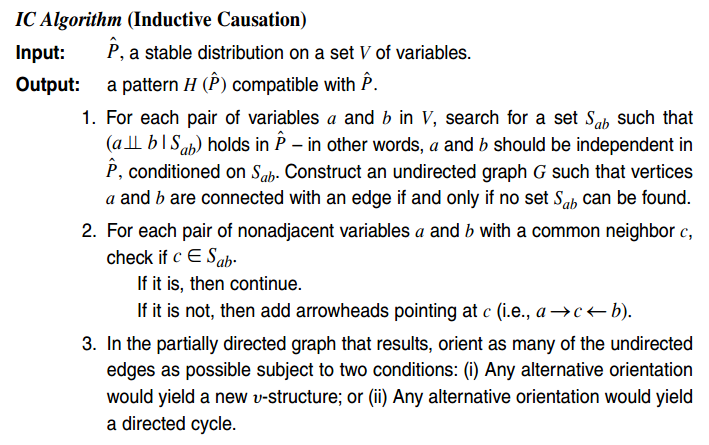
\includegraphics[scale = 0.5]{ic_algo.png}}
%\end{minipage}
%\caption{\footnotesize{\textbf{The inductive causation algorithm.  \citep{pearl2000causal}}}}
%\label{fig: ic_algo}
%\end{figure}

%\item  \begin{definition} (\textbf{\emph{Minimality}}) \citep{pearl2000causal}\\
%A latent structure $L$ is \emph{\textbf{minimal}} with respect to a class $\cL$ of latent structures if and only
%if there is no member of $\cL$ that is strictly preferred to $L$ – that is, if and only if for every $L'\in \cL$ we have $L' \equiv L$ whenever $L' \succeq L$.
%\end{definition}  

\item \begin{definition} (\textbf{\emph{Consistency}}) \citep{pearl2000causal}\\
A latent structure $L = (D, O)$ is \emph{\textbf{consistent}} with a distribution $\hat{P}$ over $O$ if $D$ can accommodate some model that generates $\hat{P}$ – that is, if there exists a parameterization $\Theta_{D}$ such that $P(O | D, \Theta_{D}) = \hat{P}$.
\end{definition}
%
%Clearly, a necessary (and sometimes sufficient) condition for $L$ to be consistent with $\hat{P}$ is that $L$ can account for all the dependencies embodied in $\hat{P}$
%\item 
% \begin{definition} (\textbf{\emph{Inferred Causation}}) \citep{pearl2000causal}\\
%Given $\hat{P}$, a variable $C$ has a \emph{\textbf{causal influence}} on variable $E$ if and only if there exists a \emph{directed path} from $C$ to $E$ in \textbf{\emph{every minimal latent structure consistent with}} $\hat{P}$.
%\end{definition} Algorithm in Figure \ref{fig: ic_algo} described an algorithm to infer causation from $\hat{P}$.
%
\item  \begin{definition}(\textbf{\emph{Faithfulness}} and \textbf{\emph{Causal Minimality}}) \citep{peters2017elements}\\
Consider a distribution $P_{\mb{X}}$ and a DAG $\cG$.
\begin{enumerate}
\item $P_{\mb{X}}$ is \textbf{\emph{faithful}} to the DAG $\cG$ if
\begin{align*}
A \indep B \;|\; C \Rightarrow A\; \indep_{\cG}\; B\; | \;C
\end{align*}
 for all disjoint vertex sets $A, B, C$.
 
\item A distribution satisfies \textbf{\emph{causal minimality}} with respect to $\cG$ if it is \textbf{Markovian} with respect to $\cG$, but not to \emph{any} proper \emph{subgraph} of $\cG$
\end{enumerate}
\end{definition}

\item \begin{proposition} (\emph{\textbf{Faithfulness implies causal minimality}}) \citep{peters2017elements}\\
 If $P_{\mb{X}}$ is faithful and Markovian with respect to $\cG$, then causal minimality is satisfied.
\end{proposition}
\end{itemize}

\newpage
\section{Structural Causal Models}
\subsection{Definitions}
\begin{figure}
\begin{minipage}[t]{1\linewidth}
  \centering
  \centerline{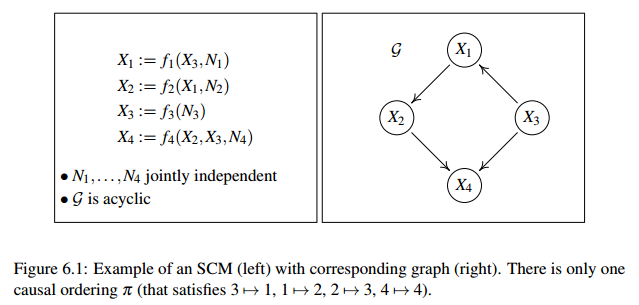
\includegraphics[scale = 0.5]{scm_example.png}}
\end{minipage}
\caption{\footnotesize{\textbf{The example of DAG created based on SCM \citep{peters2017elements}}}}
\label{fig: scm_example}
\end{figure}
\begin{itemize}
\item  \begin{definition} (\textbf{\emph{Structural causal models (SCMs})}) \citep{peters2017elements}\\
A \textbf{SCM} $\mathfrak{C}:= (S, P_{\mb{N}})$ with graph $\cG=(\cV, \cE)$ consists of a collection $S$ of $d$ \emph{\textbf{(structural) assignments}}:
\begin{align}
X_{s} &:= f_{s}(X_{\pi(s)}, N_s), \quad s=1,\ldots, d \label{eqn: scm}
\end{align} where $X_{\pi(s)}$ are called \textbf{parents} of $X_s$; and a joint distribution $P_{\mb{N}} = \prod_{s=1}^{d}P_{N_{s}}$ over the noise variables, which we require to be \underline{\emph{\textbf{jointly independent}}}.

The $\cG=(\cV, \cE)$ of a SCM is obtained by creating one vertex for each $X_s$ and drawing \textbf{directed edges} from each parent in $X_{\pi(s)}$ to $X_s$, that is, from each variable $X_k$ occurring on the right-hand side of equation \eqref{eqn: scm} to $X_s$. $\cG$ is a  \textbf{directed acyclic graph (DAG)}.

We sometimes call the elements of $X_{\pi(s)}$ not only parents but also \underline{\textbf{\emph{direct causes}}} of $X_s$, and we call $X_s$ a \underline{\textbf{\emph{direct effect}}} of each of its direct causes. SCMs are also called (\textbf{\emph{nonlinear}}) \textbf{\emph{SEMs}}.
\end{definition}

Structural assignments \eqref{eqn: scm} should be thought of as a set of \textbf{assignments} or \textbf{functions} (rather than a set of mathematical equations) that tells us how certain variables determine others. This is the reason why we prefer to avoid the term \emph{\textbf{structural equations}}, which is commonly used in the literature.

\begin{figure}
\begin{minipage}[t]{1\linewidth}
  \centering
  \centerline{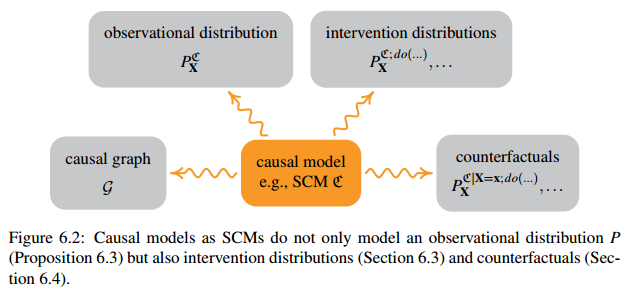
\includegraphics[scale = 0.6]{scm_causal_observe_intervene_counter.png}}
\end{minipage}
\caption{\footnotesize{\textbf{The structural cause models connect to observational, interventional and counterfactual analysis \citep{peters2017elements}}}}
\label{fig: scm_causal_observe_intervene_counter}
\end{figure}

\item SCMs are the key for formalizing \emph{causal reasoning} and \emph{causal learning}. A SCM entails an \textbf{observational distribution}. But unlike usual probabilistic models, they additionally entail \underline{\textbf{\emph{intervention distributions}}} and \underline{\textbf{\emph{counterfactuals}}}:
\begin{proposition}(\textbf{Entailed distributions}) \citep{peters2017elements}\\
A SCM $\mathfrak{C}$ defines a \textbf{unique} distribution over the variables $\mb{X} = (X_1, \ldots, X_d)$ such that $X_s = f_{s}(X_{\pi(s)}, N_s)$, in distribution, for
$s=1,\ldots, d$. We refer to it as the \textbf{entailed distribution} $P_{\mb{X}}^{\mathfrak{C}}$ and sometimes write $P_{\mb{X}}$.
\end{proposition}

\item In continous-time, we can rewrite the SCM in \eqref{eqn: scm} as a set of \emph{differential equations}. And the analysis on causality can be done at stationary state.
\end{itemize}

\subsection{Cause-effect models}
\begin{itemize}
\item A simple bivariate SCM is also called a \textbf{cause-effect model}.
 \begin{definition} (\textbf{Cause-Effect models}) \citep{peters2017elements}\\
A \textbf{SCM} $\mathfrak{C}$ with graph $\cG: C \rightarrow E$ consists of two assignments:
\begin{align}
C &:= N_{C},  \label{eqn: scm_1}\\
E &:= f_{E}(C, N_E), \label{eqn: scm_2}
\end{align} where $N_E \indep N_C$, that is, $N_E$ is independent of $N_C$. Let $C \in \cC$ and $E \in \cE$ so that $f_E: \cC \rightarrow \cE \in \cE^{\cC}$.
\end{definition}

%\item  In this model, we call the random variables $C$ the \textbf{cause} and $E$ the \textbf{effect}. Furthermore, we call $C$ a \emph{\textbf{direct cause}} of $E$, and we refer to $C \rightarrow E$ as a \textbf{causal graph}. SCM is used to study the cause-effect relationship. Given the noise distributions $P_{N_C}$ and $P_{N_E}$ and function $f$, we can generate effect $E$ from SCM. SCM thus entails a joint distribution $P_{C,E}$ over $C$ and $E$.

\item Note that from \eqref{eqn: scm_2}, $E$ is deterministic given $C$ and noise assignment  $n_E$. Thus we can view $n_E$ as choosing randomly from space of functions $\cE^{\cC}$. Based on this perspective, we can represent \eqref{eqn: scm_2} in \textbf{canonical} form 
\begin{align*}
E &:= N_{E}(C).
\end{align*} This form implies that the choice of noise factor $N_E$ determine the function $f_{E} \in \cE^{\cC}$.

\item There are two types of \emph{causal statements} entitled by SCM \eqref{eqn: scm_1} and \eqref{eqn: scm_2}:
\begin{enumerate}
\item The behavior of the system under \textbf{potential interventions}, i.e. $P_{E}^{do(C=c)} = P_{E|C=c}$. 

The \emph{\textbf{interventional causal implications}} of the SCM are completely determined by the \textbf{marginal distributions} of each component of the vector-valued noise variable $N_E$ even though the SCM includes a precise specification of $P_{N_E}$. 

\item The \textbf{counterfactual} statement. The counterfactual statements depend not only on the marginal distributions of the components of the
noise variable $N_E$, but also on the statistical dependences between the outputs of functions $f_{E} \in \cE^{\cC}$  defined in \eqref{eqn: scm_2}.
\end{enumerate}


\end{itemize}


\subsection{Intervention}
\begin{figure}
\begin{minipage}[t]{1\linewidth}
  \centering
  \centerline{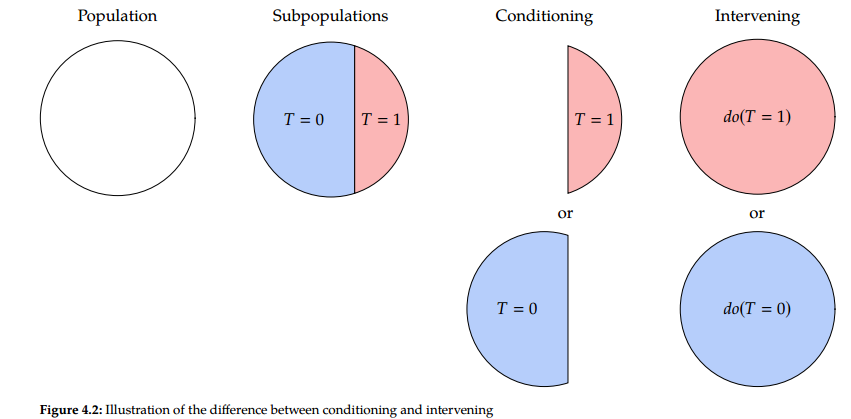
\includegraphics[scale = 0.5]{intervention_condition.png}}
\end{minipage}
\caption{\footnotesize{\textbf{The condition and intervention are not the same  \citep{neal2020introduction}}}}
\label{fig: intervention_condition}
\end{figure}
In causal inference, we are often interested in the system’s behavior under an \emph{\textbf{intervention}}. The intervened system induces \textbf{another distribution}, which usually differs from the \textbf{observational distribution}. If any type of intervention can lead to an arbitrary \textbf{change of the system}, these two distributions become \emph{\textbf{unrelated}} and instead of studying the two systems jointly we may consider them as \emph{two separate systems}. This motivates the \textbf{idea} that after an intervention \emph{only parts of the data-generating process change}. 

The first thing that we will introduce is a mathematical operator for intervention, the \underline{\textbf{\emph{do}-operator}}. For example, when we replace the assignment \eqref{eqn: scm_2} by $E := 4$. This is called a \textbf{(hard) intervention} and is \emph{denoted} by $do(E := 4)$.  

\begin{itemize}
\item \begin{definition}  (\textbf{\emph{Intervention distribution}}) \citep{peters2017elements}\\
Consider an SCM $\mathfrak{C} := (S, P_{\mb{N}})$ and its entailed distribution $P_{\mb{X}}^{\mathfrak{C}}$. We \textbf{\emph{replace}} one (or several) of the \emph{\textbf{structural assignments}} to obtain a \textbf{new SCM} $\widehat{\mathfrak{C}}$. Assume that we replace the assignment for $X_k$ by
\begin{align*}
\widehat{X}_{k} &:= \widehat{f}_{k}(\widehat{X}_{\pi(k)}, \widehat{N}_k).
\end{align*}
We then call the entailed distribution of the new SCM an \underline{\textbf{\emph{intervention distribution}}} and say that the variables whose structural assignment we have replaced have been \textbf{intervened} on. We denote the new distribution by
\begin{align*}
P_{\mb{X}}^{\widehat{\mathfrak{C}}} &:=  P_{\mb{X}}^{\mathfrak{C}: do\paren{\widehat{X}_{k} := \widehat{f}_{k}(\widehat{X}_{\pi(k)}, \widehat{N}_k)}}.
\end{align*}  The set of noise variables in $\widehat{\mathfrak{C}}$ now contains both some "new" $ \widehat{N}$’s and some "old" $N$’s, all of which are required to be \textbf{jointly independent}.

When $\widehat{f}_{k}(\widehat{X}_{\pi(k)}, \widehat{N}_k)$ puts a point mass on a real value $a$, we simply write  $P_{\mb{X}}^{\mathfrak{C}: do(X_k := a)}$
and call this an \textbf{\emph{atomic intervention}}. An intervention with $\widehat{X}_{\pi(k)} = X_{\pi(k)}$, that is, where direct causes \emph{remain} direct causes, is called \emph{\textbf{imperfect}}.  This is a special case of a \textbf{\emph{stochastic intervention}} [Korb et al., 2004], in which the marginal distribution of the intervened variable has positive variance. 

We require that the new SCM $\widehat{\mathfrak{C}}$ have an \textbf{acyclic graph} $\widehat{\cG}_{X_k}$; the set of allowed interventions thus depends on the graph induced by $\mathfrak{C}$.
\end{definition}
\end{itemize}

\subsubsection{\emph{do}-operators}
\begin{itemize}
\item   The \textbf{\emph{do}-operator} is different from \textbf{conditioning}. Conditioning on $T = t$ just means that we are restricting our \emph{focus} to the \emph{\textbf{subset}} of the population to those who have treatment $T=t$. In contrast, an intervention would be to take \textbf{\emph{the whole population}} and give everyone treatment $T=t$.

\item The notation of \emph{do}-operator is commonly used in graphical causal models, and it has equivalents in \textbf{potential outcomes} notation.
\begin{align}
P(Y(t) = y) &:= P(Y = y \,|\, do(T = t)) := P(y \,|\, do(t)) := P_{Y}^{do(T=t)}  \label{eqn: do_dist}
\end{align} The \textbf{\emph{ATE (average treatment effect)}} can be written as 
\begin{align}
\E{}{Y(1) - Y(0)} &= \E{}{Y\,|\, do(T=1)} -  \E{}{Y\,|\, do(T=0)} \label{eqn: ate_do}
\end{align} As discussed above, the distribution $P_{Y}^{do(T=t)}$ is not conditional distribution $P_{Y|T=t}$ but full distribution of $Y$ under intervention $T=t$. Denote the corresponding density of interventional distribution $p^{do(T=t)}(c)$.


%\underline{\textbf{\emph{Interventional distributions}}} such as $P(Y \,|\, do(T = t))$ are conceptually quite different from the \emph{observational distribution} $P(Y)$ or $P(Y, T)$. We can obtain $P(Y)$ or $P(Y, T)$ without carrying out experiments.

\item If an expression $Q$ with \emph{do}-operator can be converted to without \emph{do} in it, this expression is \textbf{\emph{identifiable}}.  We will refer to an
\emph{estimand} as a \emph{\textbf{causal estimand}} when it contains a \emph{do}-operator, and we refer to an estimand as a \emph{\textbf{statistical estimand}} when it doesn’t contain a \emph{do}-operator.

\item Whenever, $do(T=t)$ appears \textbf{after} the conditioning bar, it means that everything in that expression is in the \emph{\textbf{post-intervention}} world where the
intervention $do(T=t)$ occurs.  

For example $\E{}{Y| do(T=t), Z=z}$ refers to the expected outcome in the subpopulation where $Z=z$ after the whole subpopulation has taken treatment $T=t$.  On the other hand,  $\E{}{Y| Z=z}$ simply refers to the expected value in the (\emph{pre-intervention}) population where individuals take whatever treatment they would normally take ($T$)). 

\item Instead of hard intervention, we can have $do(E=g_{E}(C) + \hat{N}_{E})$, which keeps a functional dependence on $C$ but changes the noise distribution. This is an example of a \textbf{soft intervention}.

\item Intervention on effect variables $E$ will \textbf{not} change the distribution of cause variables $C$. $P_{C}^{do(E=e)} = P_{C}^{\cC}$ for all $e$. On the other hand, intervention on the "cause" variables $C$ will change the distribution of "effect" variables $E$. For instance, in \eqref{eqn: scm_1} and \eqref{eqn: scm_2} let $N_E$ and $N_C$ be standard normal distributed $N(0,1)$. Let $E = 4 C + N_{E}$. Then $P_{E}^{\cC} = N(0, 17) \neq P_{E}^{do(C=2)} = N(8, 1) = P_{E|C=2}^{\cC}$. 

The \textbf{asymmetry} between cause and effect can also be formulated as an \textbf{independence statement}. Intervention on effect variables $E$ will break the dependency between $C$ and $E$ so that $(C \indep E)_{do(E=e)}$ under intervention. %It is not sure when intervention on $C$.
\end{itemize}

\subsubsection{\emph{do}-calculus}
\begin{itemize}
\item 
\begin{proposition}(\textbf{Rules of do Calculus})\citep{pearl2000causal}  \\
Let $\cG$ be the directed acyclic graph associated with a causal model as defined in \eqref{eqn: scm_1}, \eqref{eqn: scm_2}, and let $P(\cdot)$ stand for the probability distribution induced by that model. For any \textbf{disjoint} subsets of variables $X$, $Y$, $Z$, and $W$, we have the following rules.
\begin{enumerate}
\item (\textbf{Insertion/deletion of observations}):
\begin{align}
p(y| \hat{x}, z, w)&= p(y| \hat{x},  w) \quad \text{if }(Y \indep Z | X, W)_{\widehat{\cG}_{X}} \label{eqn: do_del_ob}
\end{align} where $\hat{x} := do(X=x)$ and $\widehat{\cG}_{X}$ is induced sub-graph under intervention $\hat{x}$.

\item (\textbf{Action/observation exchange}):
\begin{align}
p(y| \hat{x}, \hat{z}, w)&= p(y| \hat{x}, z, w) \quad \text{if }(Y \indep Z | X, W)_{\widehat{\cG}_{X, Z}}  \label{eqn: do_exch_act_ob}
\end{align} where $\widehat{\cG}_{X,Z}$ is induced sub-graph under intervention $\hat{x}, \hat{z}$.

\item  (\textbf{Insertion/deletion of actions}):
\begin{align}
p(y| \hat{x}, \hat{z}, w)&= p(y| \hat{x},  w) \quad \text{if }(Y \indep Z | X, W)_{\widehat{\cG}_{X, Z(W)}} \label{eqn: do_del_act}
\end{align} where $Z(W)$ is the set of $Z$-nodes that are \textbf{not ancestors} of any $W$-node in $\widehat{\cG}_{X}$.
\end{enumerate}
\end{proposition}

The equation \eqref{eqn: do_del_ob} is based on d-separation of graphical model \textbf{after the intervention} $do(X=x)$. The equation \eqref{eqn: do_exch_act_ob} provides a condition for an \emph{\textbf{external intervention}} $do(Z=z)$ to have the same effect on $Y$ as the \emph{\textbf{passive observation}} $Z=z$. \eqref{eqn: do_del_act} provides conditions for \emph{deleting} (or introducing) an external intervention $do(Z=z)$ introduces no new association
that can affect the probability of $Y=y$. $Z(W)$ is an additional constraint set to prevent inducing association by conditioning on the descendants of \emph{colliders}.

\item 
\begin{theorem}(\textbf{Do-calculus are complete}) \citep{peters2017elements}\\
The following statements hold.
\begin{enumerate}
\item The rules are \textbf{complete}; that is, all identifiable intervention distributions can
be computed by an iterative application of these three rules \citep{huang2006pearl, shpitser2006identification};

\item In fact, there is an algorithm  that is guaranteed \citep{huang2006pearl, shpitser2006identification} to find all identifiable
intervention distributions. 

\item There is a necessary and sufficient graphical criterion for identifiability of
intervention distributions \citep{shpitser2006identification}, based on
so-called hedges \citep{huang2006pearl}.
\end{enumerate}
\end{theorem}
\end{itemize}

\subsection{Counterfactuals}
Another possible modification of an SCM changes all of its noise distributions. Such a change can be induced by observations and allows us to answer \textbf{counterfactual questions} such as "What if i did this, what would the outcome be ?". The \textbf{counterfactual outcome} is the result of \textbf{intervention on alternative cause} in SCM \emph{\textbf{given the observation of current cause and effect}}.

\begin{itemize}
\item \begin{definition} (\textbf{\emph{Counterfactuals}})  \citep{peters2017elements} \\
Consider an SCM $\mathfrak{C} := (S, P_{\mb{N}})$ over nodes $\mb{X}$. Given some observations $\mb{x}$, we define a \underline{\textbf{\emph{counterfactual}}} SCM by \textbf{replacing} the distribution of \emph{\textbf{noise variables}}:
\begin{align*}
\mathfrak{C}_{\mb{X} = \mb{x}} &= \paren{S, P_{\mb{N}}^{\mathfrak{C}|_{\mb{X} = \mb{x}}}}
\end{align*}
where $P_{\mb{N}}^{\mathfrak{C}|_{\mb{X} = \mb{x}}} = P_{\mb{N} | \mb{X} = \mb{x}}$. The new set of noise variables \textbf{need not be jointly independent} anymore. Counterfactual statements can now be seen as \emph{do}-statements in the \emph{new counterfactual SCM}.
\end{definition} This definition can be generalized such that we observe not the full vector X = x
but only some of the variables. 


\begin{figure}
\begin{minipage}[t]{1\linewidth}
  \centering
  \centerline{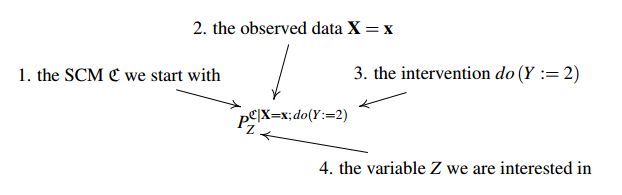
\includegraphics[scale = 0.6]{counterfactual_construction.png}}
\end{minipage}
\caption{\footnotesize{\textbf{The diagram illustration of steps in counterfactual analysis.  \citep{peters2017elements}}}}
\label{fig: counterfactual_construction}
\end{figure}

\item The steps for counterfactual analysis in Figure \ref{fig: counterfactual_construction}:
\begin{enumerate}
\item Given SCM $\mathfrak{C}$, we can first \textbf{condition} on \emph{observations} $\mb{X} = \mb{x}$ to update the distribution over the noise variables.

\item Next, we calculate the effect of \textbf{intervention} on alternative treatment $do(Y := 2)$ for the SCM. 

\item  Finally, we can compute the probablilty of outcome $Z$ conditioned on both observations and do-operator, i.e. $P_{Z}^{\mathfrak{C}|\mb{X}=\mb{x}, do(Y=2)}$ as the counterfactural outcome.
\end{enumerate}

\item Counterfactual statements depend strongly on the \underline{\textbf{structure of the SCM}}. Two SCMs can induce the \emph{same graph}, \emph{observational distributions}, and \emph{intervention distributions} but \emph{entail \textbf{different counterfactual statements}}.  We will call those SCMs "\emph{probabilistically and interventionally equivalent}" but not "\emph{counterfactually equivalent}". 

In this sense, causal graphical models are \emph{not \textbf{rich} enough} to predict \textbf{counterfactuals}.

\begin{definition}(\textbf{\emph{Equivalence of causal models}})  \citep{peters2017elements}\\
 Two models are called
 \begin{align*}
 \{\text{probabilistically / interventionally / counterfactually}\}\text{ equivalent}
 \end{align*}
if they entail the same $\{\text{obs. / obs. \textbf{and} int. / obs., int., \textbf{and} counter.}\}$ distributions.
\end{definition}

\end{itemize}


\subsection{Truncated Factorization}
\begin{itemize}
\item \begin{proposition} (\emph{\textbf{Truncated Factorization}})  \citep{pearl2000causal, peters2017elements, neal2020introduction}\\
We assume that $p$ and $\cG$ satisfy the Markov assumption and modularity. Given, a set of \textbf{intervention} nodes $S$, if $\mb{x}$ is \textbf{consistent} with the intervention, then
\begin{align}
p(x_1, \ldots, x_{m} \,|\, do(S = s)) &= \prod_{ i\not\in S}p_i(x_i | x_{\pi(i)}) \label{eqn: truncation_intervention_prod}
\end{align}
Otherwise, $p(x_1, \ldots, x_{m} | do(S = s)) = 0$.
\end{proposition} That is for all factors related to $X_i \in S$, the values are set to be $1$ due to intervention. In other words, the
factors for \eqref{eqn: truncation_intervention_prod} have been \emph{truncated} compared to \eqref{eqn: dag_graph_factorization}.

\item An \emph{alternative interpretation} is that for any SCM $\widehat{\mathfrak{C}}$ obtained from $\mathfrak{C}$ by intervening on some $X_i$, we have the following \emph{invariance} statement:
\begin{align}
p^{\widehat{\mathfrak{C}}}(x_j \,|\,x_{\pi(j)}) = p^{\mathfrak{C}}(x_j \,|\,x_{\pi(j)}), \quad \forall\, j \neq i.  \label{eqn: auto_intervention}
\end{align} The equation in \eqref{eqn: auto_intervention} shows that \emph{causal relationships} are \emph{\textbf{autonomous}} under interventions: if we intervene on a variables, the other mechanisms remain \textbf{\emph{invariant}}. 

\item Truncated factorization is also called \emph{\textbf{G-computation formula}} \citep{imbens2015causal} and \textbf{manipulation theorem}.
\end{itemize}


\section{The Principle of Independent Mechanisms}
Given two variables $A, T$ and their joint distribution $p(a, t)$, how to determine the causal structure ($A\rightarrow T$ or $T\rightarrow A$) ?  A first idea is to consider the \textbf{effect of interventions}. If we can change the value of $A$, how would the value of $T$ change ? Here we assume that \emph{the physical mechanism} $p(t | a)$
responsible for producing $T$ given $A$. If $A\rightarrow T$ is a causal relationship, this would hold true independent of the distribution from $A$, $p(a)$. 

Specifically, if $A\rightarrow T$ is the correct causal structure, then
\begin{enumerate}
\item it is in principle possible to perform a \underline{\textbf{\emph{localized intervention}}} on $A$, in other
words, to change $p(a)$ without changing $p(t | a)$, and

\item $p(a)$ and $p(t | a)$ are \underline{\textbf{\emph{autonomous}}}, \underline{\textbf{\emph{modular}}}, or \textbf{\emph{invariant}} mechanisms or objects in the world.
\end{enumerate}
\begin{itemize}
\item 
 In the \textbf{causal factorization} $p(a, t) = p(t|a) p(a)$, we would expect that the \emph{conditional density} $p(t|a)$ (viewed as a \emph{\textbf{function}} of $t$ and $a$) provides no information about the \emph{\textbf{marginal} density function} $p(a)$.  This holds true if $p(t|a)$ is a model of a \textbf{\emph{physical mechanism}} that does not care about what distribution $p(a)$ we feed into it. This is called the \textbf{independence of cause and mechanism}.
 
\item In previous example, we can write $A\rightarrow T$ into a SCM
\begin{align*}
A &= N_{A} \\
T &= f_{T}(A, N_{T})
\end{align*} where $N_T$ and $N_{A}$ are \textbf{statistically independent noises} $N_T \indep N_A$. 

\begin{figure}
\begin{minipage}[t]{1\linewidth}
  \centering
  \centerline{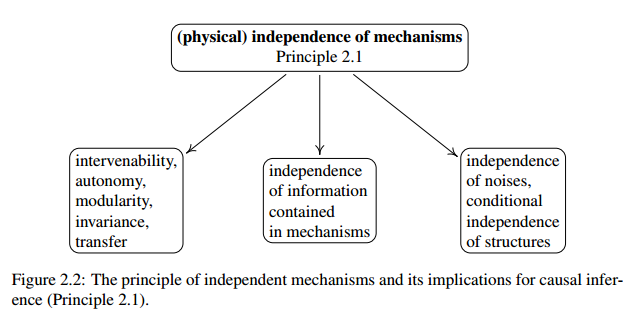
\includegraphics[scale = 0.55]{indep_mech.png}}
\end{minipage}
\caption{\footnotesize{\textbf{The independent mechanism priniciple  \citep{peters2017elements}}}}
\label{fig: indep_mech}
\end{figure}


\item \begin{principle}(\textbf{Independent mechanisms}) \citep{peters2017elements} \\
The causal generative process of a system’s variables is composed of \textbf{autonomous modules} that do not inform or influence each other.

In the probabilistic case, this means that the \textbf{conditional distribution} of each variable given its \textbf{causes} (i.e., its mechanism) does \textbf{not inform or influence} the other conditional distributions. In case we have only two variables, this reduces to an \textbf{independence} between the \textbf{cause} distribution and the \textbf{mechanism} producing the effect distribution.
\end{principle}

\item% Recall the \textbf{Ignorability} or \textbf{Exchangeability} in Potential Outcomes theory
\begin{assumption} (\textbf{Ignorability / Exchangeability}) \citep{neal2020introduction}
\begin{align}
(Y(1), Y(0)) \indep T  \label{eqn: Ignorability}
\end{align}
\end{assumption} Note that $(Y(1), Y(0))$ describes the mechansim and $P_{Y(t)} = P_{Y}^{do(T=t)} = P_{Y|T=t}$ when $T\rightarrow Y$ is a causal structure. This assumption is the same as the independent mechanisms principle.

\item The independent mechanism assumption implies that we can \textbf{change one mechanism without affecting the others}, -- or, in causal terminology, we
can \textbf{intervene} on one mechanism without affecting the others. An assumption such as this one is often implicit to \textbf{justify} the possibility of interventions in
the first place, but one can also view it as a more general basis for causal reasoning and causal learning.

\item The existence of an \textbf{invariant} mechanism under local intervention can be used in domain adapation and transfer learning \citep{peters2017elements}.

\item It is important to distinguish between two levels of information: an \textbf{effect} contains information about its cause, but the \textbf{mechanism} that \textbf{\emph{generates}} the effect from its cause contains \emph{no} information about the mechanism generating the cause. ($P_{Y(1), Y(0)} = P_{Y}^{do(T=0,1)}  \neq P_{Y}$)
\end{itemize}

\section{Controlling confounding bias}
\begin{itemize}
\item \emph{\textbf{Covariates}} or \emph{\textbf{confounding factors}} are variables other than the cause and effect variables of interest but have impact on them.
\begin{definition} (\textbf{\emph{Confounding}}) \citep{peters2017elements} \\
Consider an SCM  $\mathfrak{C}$ over nodes $\cV$ with a directed path from $X \rightarrow Y$, $X, Y \in \cV$. The causal effect from $X$ to $Y$ is called \emph{\textbf{confounded}} if
\begin{align}
p^{\mathfrak{C}: do(X=x)}(y) &\neq p^{\mathfrak{C}}(y | x). \label{eqn: confounding}
\end{align}
Otherwise, the causal effect is called \underline{\textbf{\emph{unconfounded}}}.
\end{definition}

\item In order to account for the influence of confounder, we should \textbf{partition} the population into groups that are \emph{\textbf{homogeneous}} relative to \emph{confounder} $Z$, assessing the effect of $X$ on $Y$ in each homogeneous group, and then averaging the results. This process is called \underline{\textbf{\emph{covariate}}} \underline{\textbf{\emph{adjustment}}}. This is the idea behind the \emph{\textbf{Adjustment Formula}}  \citep{imbens2015causal}.

\item \emph{\textbf{Confounder}} should be distinguished from the \emph{\textbf{collider}}: confounders \emph{\textbf{need}} to be \textbf{controlled for} when estimating causal associations, while collider should be \textbf{avoided} during the conditioning.
\end{itemize}



This section discuss the process of \textbf{choosing} adjustment set using causal structure.
\subsection{The Back-door Adjustment}
Assume we are given a \emph{\textbf{causal diagram}} $\cG$, together with \emph{nonexperimental} data on a subset $V$ of observed variables in $\cG$, and suppose we wish to estimate what effect the interventions $do(X = x)$ would have on a set of response variables $Y$, where $X$ and $Y$ are two subsets of $V$. In other words, we seek to estimate $P(y\,|\, do(x))$ from a sample estimate of $P(v)$, given the assumptions encoded in $\cG$.

The \textbf{\emph{back-door adjustment}} or \emph{back-door criterion} \citep{pearl2000causal} is a simple graphical test that can be applied directly to the causal diagram in order to test if a set $Z \subseteq V$ of variables is sufficient for identifying $P(y \,|\,do(x))$.

\begin{figure}
\begin{minipage}[t]{1\linewidth}
  \centering
  \centerline{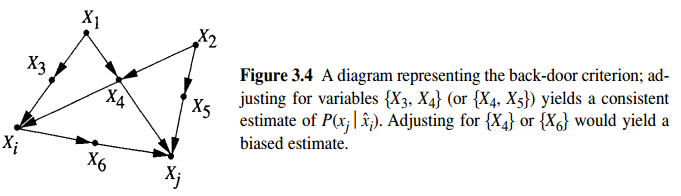
\includegraphics[scale = 0.6]{backdoor.png}}
\end{minipage}
\caption{\footnotesize{\textbf{The back-door adjustment  \citep{pearl2000causal}}}}
\label{fig: backdoor}
\end{figure}

\begin{itemize}
\item 
\begin{definition}(\textbf{Back-Door}) \citep{pearl2000causal}\\
A set of variables $Z$ satisfies the \emph{\textbf{back-door criterion}} relative to an \emph{\textbf{ordered}} pair of variables $(X_i \rightarrow X_j)$ in a DAG $\cG$ if:
\begin{enumerate}
\item \emph{\textbf{no}} node in $Z$ is a \emph{\textbf{descendant}} of $X_i$; and
\item $Z$ \emph{\textbf{blocks every path}} between $X_i$ and $X_j$ that contains an arrow \textbf{\emph{into}} $X_i$.
\end{enumerate}
Similarly, if $X$ and $Y$ are two \textbf{disjoint} subsets of nodes in $\cG$, then $Z$ is said to satisfy \textbf{\emph{the back-door criterion}} relative to $(X, Y)$ if it satisfies the criterion relative to \emph{any pair} $(X_i, X_j)$ such that $X_i \in X$ and $X_j \in Y$.
\end{definition} 

\item The first condition makes sure \emph{\textbf{no descendant of the treatment is included}}. The second condition requires that \emph{only paths with arrows \textbf{pointing at} $X_i$ be blocked}; these paths can be viewed as \textbf{entering} $X_i$ through the \emph{\textbf{back door}}.

%\item From graphical model point of view, $Z$ satisfies the back-door criterion relative to $(X, Y)$ $\Leftrightarrow$ The one directional $X\rightarrow Y$ are \textbf{d-separated} given $Z$ but not vice versa. (There is no active trails from $X$ to $Y$ given $Z$).

\item  Satisfying the back-door criterion makes $Z$ a \emph{\textbf{\underline{sufficient} adjustment set}}. The main insight of the graphical approach to covariate adjustment is that the adjustment set must \textbf{block all \emph{noncausal} paths} \textbf{without blocking} any \emph{\textbf{causal}} paths between $X$ and $Y$. 

\item $X$ and $Y$ are \textbf{not d-separated} given $Z$ since the \emph{front-door path} $X \rightarrow Y$ is not blocked. 

\item \begin{theorem} (\textbf{Back-Door Adjustment}) \citep{pearl2000causal, neal2020introduction}\\
If a set of variables $Z$ satisfies the back-door criterion relative to $(X, Y)$, then the causal effect of $X$ on $Y$ is \textbf{identifiable} and is given by the formula
\begin{align}
P(y\,|\, do(x)) &= \sum_{z}P(y\,|\,x,  z)P(z) \label{eqn: back_door_adjustment}
\end{align}
\end{theorem} To see why this works we need to know that $P(z| do(x)) = P(z)$ since by back-door criterion, $Z$ has no descendant of $X$. Also $P(y\,|\,do(x),  z) = P(y\,|\,x,  z)$ since $Z$ blocks all paths from $X$ to $Y$, so by modularity 

\item The summation in \eqref{eqn: back_door_adjustment} represents the standard formula obtained under adjustment for $Z$; variables $X$ for which the equality in \eqref{eqn: back_door_adjustment} is valid were named "\emph{\textbf{conditionally ignorable} given $Z$}" as in \citep{imbens2015causal}.
\begin{align*}
(Y(1), Y(0)) \indep X \;|\; Z 
\end{align*}

\item Using back-door criterion, we can choose set $Z$ that blocks the non-collider path from $Y$ to $X$.
\end{itemize}

\subsection{Collider Bias and Why to Not Condition on Descendants of Treatment}
\begin{figure}
\begin{minipage}[t]{0.33\linewidth}
  \centering
  \centerline{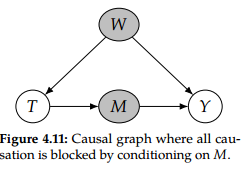
\includegraphics[scale = 0.6]{collider_bias_1.png}}
  \vspace{-5pt}
  \centerline{(a)}
\end{minipage}
\begin{minipage}[t]{0.33\linewidth}
  \centering
  \centerline{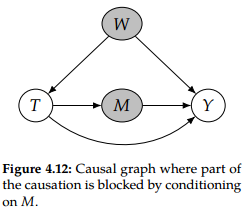
\includegraphics[scale = 0.6]{collider_bias_2.png}}
  \vspace{-5pt}
  \centerline{(b)}
\end{minipage}
\begin{minipage}[t]{0.33\linewidth}
  \centering
  \centerline{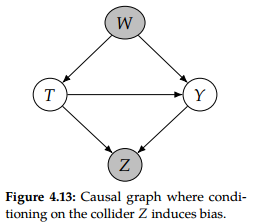
\includegraphics[scale = 0.6]{collider_bias_3.png}}
  \vspace{-5pt}
  \centerline{(c)}
\end{minipage}
\caption{\footnotesize{\textbf{The collider bias induced by conditioning on descendant of treatment \citep{neal2020introduction}}}}
\label{fig: collider_bias}
\end{figure}
There are two categories of things that could go wrong if we condition on descendants of treatment $X$:
\begin{enumerate}
\item We \textbf{block the flow of causation} from $X$ to $Y$. 

If we condition on a node that is on a directed path from $X$ to $Y$, then we block the flow of causation along that causal path. We will refer to a node
on a directed path from $X$ to $Y$ as a \underline{\emph{\textbf{mediator}}}, as it mediates the effect of $X$ on $Y$. This way we have either completely independent variables conditioned on mediator $Z$ (Figure \ref{fig: collider_bias} (a)) or we have biased estimation (Figure \ref{fig: collider_bias} (b)).

\item We \textbf{induce non-causal association} between $X$ and $Y$ if $Z$ is a collider, i.e. $X\rightarrow Z \leftarrow Y$.

If we condition on a descendant of $X$ that isn’t a mediator, it could \emph{\textbf{unblock}} a path from $X$ to $Y$ that was blocked by a collider (Figure \ref{fig: collider_bias} (c)). Conditioning on $Z$, or any descendant of $Z$ in a path like this, will induce \emph{\textbf{collider bias}}. That is, the causal effect estimate will be biased by the non-causal association that we induce when we condition on $Z$ or any of its descendants.
\end{enumerate}




\subsection{Compare to Adjustment Formula}
From above we can see that the Adjustment formula from Potential Outcome thoery is equivalent to the Back-Door Adjustment from SCMs.
\begin{align*}
 \E{}{Y_i(x) } = \E{}{Y| do(x)} &= \E{Z}{ \E{}{Y \,|x,\,Z } } \\
 &= \sum_{z}\E{}{Y \,|x,\,z } P(z) \\
  \E{}{Y| do(X=1)} -  \E{}{Y| do(X=0)} &= \E{Z}{ \E{}{Y \,|X=1,\,Z } -  \E{}{Y \,|X=0,\,Z }}
\end{align*}

Unlike the potential outcome theory, which do not know how to choose confounder $Z$. Using graphical causal models, we know how to choose a valid $Z$: we simply
choose $Z$, so that it satisfies the back-door criterion. Then, under the assumptions encoded in the causal graph, \emph{conditional exchangeability}
provably holds; the causal effect is provably \emph{identifiable}.

\newpage
\bibliographystyle{plainnat}
\bibliography{book_reference.bib}
\end{document}